\documentclass{article}
\usepackage[english,greek]{babel}
\usepackage{amsmath}
\usepackage{multirow}
\usepackage{graphicx}
\usepackage[shortlabels]{enumitem}
\usepackage{pgfplots}
\graphicspath{ {./images/} }

\newcommand{\lt}{\latintext}
\newcommand{\gt}{\greektext}

\title{Προαιρετική Εργασία
Στο Μάθημα της Αριθμητικής Ανάλυσης
}
\author{Ονοματεπώνυμο: Σταύρος Νικολαΐδης  \\  ΑΕΜ: 3975}
\date{Νοέμβριος 2021}

\begin{document}

\maketitle

\section{Πρώτη Άσκηση}

{\tiny Α}{\scriptsize Β}{\footnotesize Γ}{\small Δ}{\normalsize Ε}{\large Ζ}{\Large Η}{\LARGE Θ}{\huge Ι}{\Huge κ}{\huge λ}{\LARGE μ}{\Large ν}{\large ξ}{\normalsize ο}{\small π}{\footnotesize ρ}{\scriptsize σ}

\section{Δεύτερη Άσκηση}

\lt Normal \textit {Italics} \textbf {Bold} \\
\emph {Emphasized} \underline {Underlined} \gt

\section{Τρίτη Άσκηση}

\begin{gather*}
a^{2} + b^{2} = c^{2} \\
e^{i\pi} = -1 \\
\pi = \frac{c}{d} \\
\frac{d}{dx}\int_{a}^{x} f(s)ds = f(x) \\
f(x) = \sum_{i=0}^{\infty} \frac{f^{(i)}(0)}{i!}x^{i} \\
\lt\textbf{Ax = b}\gt \\
\| x + y \| \leq \| x \| + \| y \| \\
\end{gather*}

\begin{equation}
    \textbf{I} = \begin{pmatrix}
            1 & 0 & 0 & 0\\
            0 & 1 & 0 & 0\\
            0 & 0 & 1 & 0\\
            0 & 0 & 0 & 1
        \end{pmatrix}
\end{equation}

\begin{equation}
    \textbf{I} = \begin{bmatrix}
            1 & 0 & 0 & 0\\
            0 & 1 & 0 & 0\\
            0 & 0 & 1 & 0\\
            0 & 0 & 0 & 1
        \end{bmatrix}
\end{equation}

\begin{equation}
    \textbf{I} = \begin{Bmatrix}
            1 & 0 & 0 & 0\\
            0 & 1 & 0 & 0\\
            0 & 0 & 1 & 0\\
            0 & 0 & 0 & 1
        \end{Bmatrix}, \hspace{0.5cm}
    \textbf{I} = \begin{vmatrix}
            1 & 0 & 0 & 0\\
            0 & 1 & 0 & 0\\
            0 & 0 & 1 & 0\\
            0 & 0 & 0 & 1
        \end{vmatrix}, \hspace{0.5cm}
    \textbf{I} = \begin{Vmatrix}
            1 & 0 & 0 & 0\\
            0 & 1 & 0 & 0\\
            0 & 0 & 1 & 0\\
            0 & 0 & 0 & 1
        \end{Vmatrix}
\end{equation}


\section{Τέταρτη Άσκηση}

\begin{center}
\begin{tabular}{ l l l }
 Τέφας    & 2 & 3 \\ 
 Πήτας    & 5 & 6 \\
 Λάσκαρης & 8 & 9    
\end{tabular}
\end{center}

\begin{center}
\begin{tabular}{ | l | l | l |}
 Κοτρόπουλος    & 6 & 3 \\ 
 Πήτας          & 5 & 6 \\
 Κοτρόπουλος    & 8 & 9    
\end{tabular}
\end{center}

\begin{center}
\begin{tabular}{ | c | c | c |}
 \hline
 1 & 2 & 3 \\ \hline
 4 & 5 & 6 \\ \hline
 7 & 8 & 9 \\ \hline
\end{tabular}
\end{center}

\begin{center}
\begin{tabular}{ | c | c | c |}
 \hline
 1 & 2 & 3 \\ \hline
 4 & 5 & 6 \\ \hline
 7 & 8 & 9 \\ \hline
\end{tabular}
\end{center}

\begin{center}
\begin{tabular}{ |l|l|l| }
\hline
\multicolumn{3}{ |c| }{Μέλη ΔΕΠ Πληροφορικής} \\ \hline
Λέκτορες                   & \lt VD \gt & Δραζιώτης Κωνσταντίνος \\ \hline
\multirow{2}{*}{Επίκουροι} & \lt LN \gt & Λάσκαρης Νικόλαος \\
                           & \lt TG \gt & Τσουμάκας Γρηγόριος \\ \hline
\multirow{3}{*}{Αναπληρωτές} & TA & Τέφας Αναστάσιος \\
                             & \lt PN \gt & Πλέρος Νίκος \\
                             & \lt PA \gt & Παπαδόπουλος Απόστολος \\ \hline
\multirow{3}{*}{Καθηγητές}  & \lt KC \gt & Κοτρόπουλος Κωνσταντίνος\\
                            & \lt PI \gt  & Πήτας Ιωάννης \\
                            & \lt VI \gt & Βλαχάβας Ιωάννης \\ \hline
\end{tabular}
\end{center}

\section{Πέμπτη Άσκηση}

\begin{itemize}
  \item Τέφας
  \item Μπουζάς
  \item Μπρούζα
  \item Λάσκαρης
  \item Κοτρόπουλος
\end{itemize}

\begin{enumerate}
  \item Τέφας
  \item Μπουζάς
  \item Μπρούζα
  \item Λάσκαρης
  \item Κοτρόπουλος
  \item Πήτας
  \item Νικολαΐδης
\end{enumerate}

\begin{itemize}
\item[\textbf{(α)}] Τέφας
\item[\textbf{(β)}] Μπουζάς
\item[\textbf{(γ)}] Μπρούζα
\item[\textbf{(δ)}] Λάσκαρης
\item[\textbf{(ε)}] Κοτρόπουλος
\item[\textbf{(ζ)}] Πήτας
\item[\textbf{(η)}] Νικολαΐδης
\end{itemize}

\section{Έκτη Άσκηση}
\begin{center}
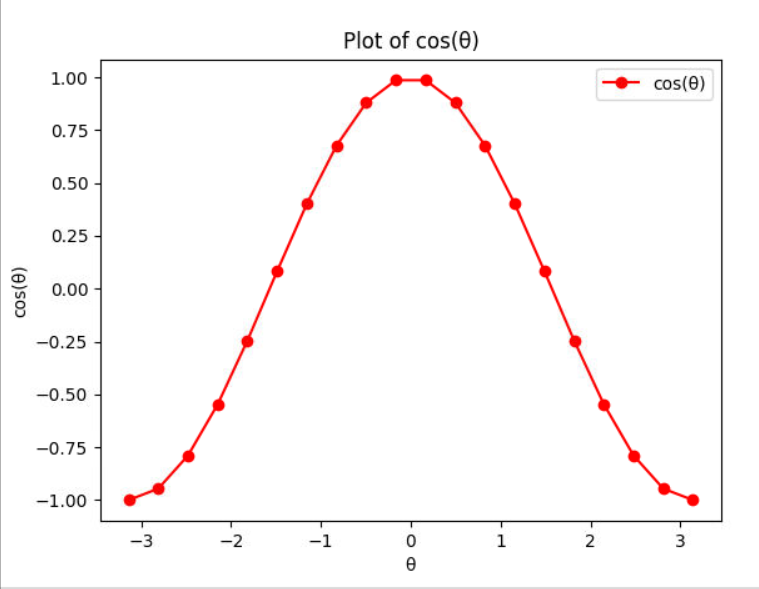
\includegraphics[width=10cm, height=7cm]{cos chart.png} \\
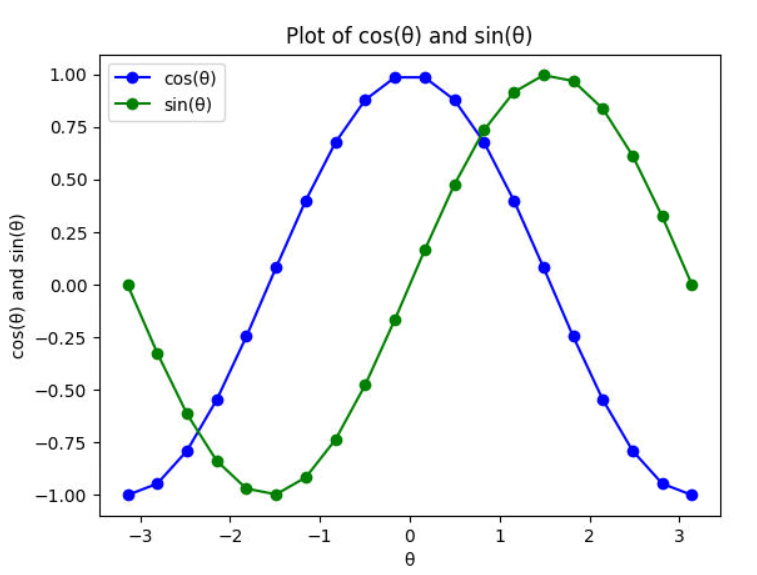
\includegraphics[width=10cm, height=7cm]{cos and sin chart.png}
\end{center}
\end{document}
